\chapter{Vorgehen}
\label{cha:vorgehen}

Dieses Kapitel beschreibt das methodische Vorgehen von der Anforderungserhebung über den Systementwurf bis zur Projektplanung.

\section{Anforderungsanalyse}
\label{sec:requirements}

Die Anforderungen wurden gemäß dem V-Modell\index{V-Modell} in funktionale, nicht-funktionale und Hardware-Anforderungen untergliedert. Jede Anforderung erhielt eine eindeutige ID, ein Akzeptanzkriterium und eine Prioritätsstufe (Muss/Soll/Kann). Die vollständige Requirements Specification liegt als separates Dokument vor.

\subsection{Funktionale Anforderungen}
\label{sec:func_req}

Tabelle~\ref{tab:func_req} zeigt die wichtigsten funktionalen Anforderungen.

\begin{table}[htb]
\centering
\renewcommand{\arraystretch}{1.3}
\captionabove[Funktionale Kernanforderungen]{Funktionale Kernanforderungen (Auszug)}
\label{tab:func_req}
\begin{tabular}{p{2cm} p{2.5cm} p{5cm} p{1.2cm}}
\toprule
\rowcolor{tableheader}
\textbf{ID} & \textbf{Name} & \textbf{Akzeptanzkriterium} & \textbf{Prio} \\
\midrule
REQ-F-001 & CO\textsubscript{2}-Messung & 400--5000\,ppm, $\pm$50\,ppm & Muss \\
REQ-F-002 & Feinstaub & 0--500\,µg/m³, 1\,µg/m³ Auflösung & Muss \\
REQ-F-003 & VOC-Messung & VOC-Index 0--500 & Muss \\
REQ-F-004 & Temperatur & 0--50\,°C, $\pm$0,5\,°C & Muss \\
REQ-F-005 & Luftfeuchte & 0--100\,\%, $\pm$3\,\% & Muss \\
REQ-F-006 & Präsenzerkennung & Reichweite 2\,m, $<$500\,ms & Muss \\
REQ-F-007 & Display-Anzeige & Alle 6 Werte sichtbar & Muss \\
REQ-F-008 & Farbcodierung & 4-Stufen-Ampel (Grün/Gelb/Orange/Rot) & Muss \\
REQ-F-009 & UI-Wechsel & 5~Screen-Designs per Button & Muss \\
\bottomrule
\end{tabular}
\end{table}

\subsection{Nicht-funktionale Anforderungen}

Wesentliche nicht-funktionale Anforderungen umfassen eine Sensor-Aktualisierungsrate von \SI{2}{\second} (REQ-NF-001), eine UI-Reaktionszeit unter \SI{200}{\milli\second} (REQ-NF-002), die Eignung für 24/7-Dauerbetrieb ohne Memory Leaks (REQ-NF-003) sowie den Betrieb über USB \SI{5}{\volt} bei maximal \SI{1}{\ampere} (REQ-NF-004). Das Gehäuse soll als 3D-Druck in PETG realisiert werden (REQ-NF-005).

\subsection{Hardware-Anforderungen}

Insgesamt wurden elf Hardware-Anforderungen (REQ-HW-001 bis REQ-HW-011) definiert, die alle Komponenten von der Mikrocontroller-Auswahl (ESP32-S3 N8R8) über die Sensorik bis zu Schutzkomponenten wie Level Shifter und Stützkondensatoren spezifizieren. Die vollständige Auflistung ist in der separaten Requirements Specification dokumentiert.

\section{Systementwurf}
\label{sec:design}

Der Systementwurf beschreibt die Hardware-Architektur und die Software-Struktur. Die vollständige Design Description liegt als separates Dokument vor.

\subsection{Hardware-Architektur}
\label{sec:hw_arch}

Das System besteht aus dem ESP32-S3 als zentraler Steuereinheit, an die fünf Sensoren und ein Display über verschiedene Schnittstellen angebunden sind. Abbildung~\ref{fig:hw_block} zeigt das Hardware-Blockdiagramm.

\begin{figure}[htb]
\centering
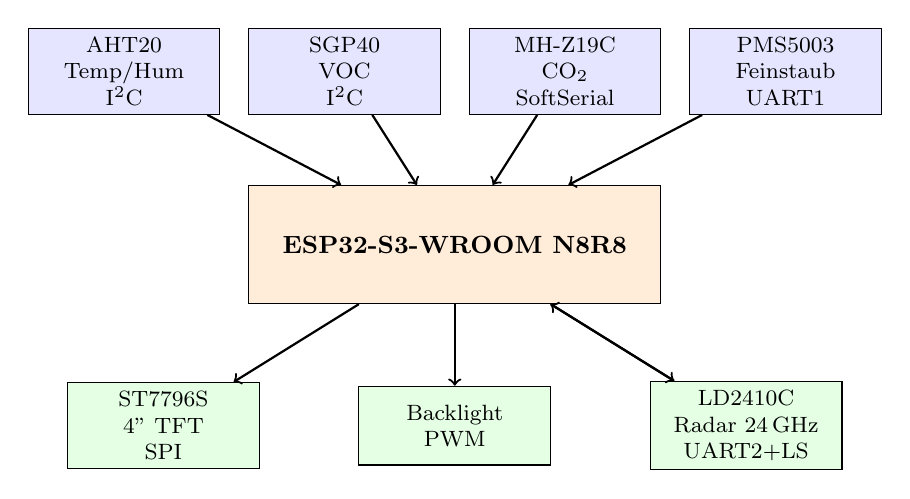
\begin{tikzpicture}[
  block/.style={rectangle, draw, fill=blue!10, text width=2.2cm, text centered, minimum height=1cm, font=\footnotesize},
  mcu/.style={rectangle, draw, fill=orange!15, text width=5cm, text centered, minimum height=1.5cm, font=\small\bfseries},
  output/.style={rectangle, draw, fill=green!10, text width=2.2cm, text centered, minimum height=1cm, font=\footnotesize},
  line/.style={->, thick}
]
% Sensors
\node[block] (aht) at (0,3) {AHT20\\Temp/Hum\\I\textsuperscript{2}C};
\node[block] (sgp) at (2.8,3) {SGP40\\VOC\\I\textsuperscript{2}C};
\node[block] (mhz) at (5.6,3) {MH-Z19C\\CO\textsubscript{2}\\SoftSerial};
\node[block] (pms) at (8.4,3) {PMS5003\\Feinstaub\\UART1};

% MCU
\node[mcu] (esp) at (4.2,0.8) {ESP32-S3-WROOM N8R8};

% Outputs
\node[output] (disp) at (0.5,-1.5) {ST7796S\\4" TFT\\SPI};
\node[output] (mos) at (4.2,-1.5) {Backlight\\PWM};
\node[output] (radar) at (7.9,-1.5) {LD2410C\\Radar 24\,GHz\\UART2+LS};

% Arrows
\draw[line] (aht) -- (esp);
\draw[line] (sgp) -- (esp);
\draw[line] (mhz) -- (esp);
\draw[line] (pms) -- (esp);
\draw[line] (esp) -- (disp);
\draw[line] (esp) -- (mos);
\draw[line] (radar) -- (esp);
\draw[line] (esp) -- (radar);
\end{tikzpicture}
\caption[Hardware-Blockdiagramm]{Hardware-Blockdiagramm des InspectAir-Systems}
\label{fig:hw_block}
\end{figure}

Die Schnittstellen-Zuordnung ist in Tabelle~\ref{tab:interfaces} zusammengefasst.

\begin{table}[htb]
\centering
\renewcommand{\arraystretch}{1.3}
\captionabove[Schnittstellen-Zuordnung]{Schnittstellen-Zuordnung der Komponenten}
\label{tab:interfaces}
\begin{tabular}{p{2.5cm} p{2cm} p{1.5cm} p{3cm} p{2.5cm}}
\toprule
\rowcolor{tableheader}
\textbf{Komponente} & \textbf{Interface} & \textbf{VCC} & \textbf{ESP32 Pins} & \textbf{Hinweis} \\
\midrule
ST7796S & SPI & 3,3\,V & 11,12,14,9,46,3 & 480$\times$320\,px \\
AHT20 & I\textsuperscript{2}C & 3,3\,V & 8 (SDA), 18 (SCL) & Pull-ups \\
SGP40 & I\textsuperscript{2}C & 3,3\,V & 8 (SDA), 18 (SCL) & Parallel AHT20 \\
MH-Z19C & SoftSerial & 5\,V & 4 (RX), 5 (TX) & 220\,µF Elko! \\
PMS5003 & UART1 & 5\,V & 16 (RX), 17 (TX) & Molex-Stecker \\
LD2410C & UART2 & 5\,V & 7 (RX), 6 (TX) & Level Shifter! \\
\bottomrule
\end{tabular}
\end{table}

\subsection{Kritische Hardware-Entscheidungen}
\label{sec:hw_decisions}

\paragraph{Stützkondensatoren:} MH-Z19C und LD2410C verursachen bei Messvorgängen Stromspitzen, die ohne Pufferung zu Spannungseinbrüchen auf dem 5\,V-Rail und damit zu Systemabstürzen führen. Die Lösung sind \SI{220}{\micro\farad} Elektrolytkondensatoren (25\,V) direkt an VCC/GND beider Sensoren.

\paragraph{Keramikkondensatoren:} Zusätzlich werden 100\,nF Keramikkondensatoren an den 3,3\,V-Rails des Displays und des ESP32 eingesetzt, um hochfrequente Störungen zu filtern und die Spannungsversorgung zu stabilisieren.

\paragraph{Level Shifter:} Der LD2410C sendet seine TX-Signale mit 5\,V-Pegel. Da die ESP32-GPIOs maximal 3,3\,V tolerieren, ist ein bidirektionaler Level Shifter (TXS0108E) zwischen Radar-TX und ESP32-GPIO\,7 zwingend erforderlich. Ohne diesen wird der ESP32 beschädigt.

\paragraph{SoftwareSerial:} Der ESP32-S3 hat nur zwei Hardware-UARTs (UART0 für USB-Monitor, UART1 für PMS5003). Für den dritten UART-Sensor (MH-Z19C) wird daher EspSoftwareSerial (v8.2.0) auf GPIO\,4/5 bei \SI{9600}{Baud} eingesetzt.

\paragraph{Backlight-Steuerung:} Das Display-Backlight wird direkt über GPIO\,3 mit PWM (44,1\,kHz) gesteuert. Der ESP32-S3 kann den Backlight-Pin des ST7796S direkt ansteuern, da dieser nur wenige mA benötigt.

\subsection{Software-Architektur}
\label{sec:sw_arch}

Die Software folgt einem dreischichtigen Architekturmodell:

\begin{itemize}[nosep]
\item \textbf{Application Layer} (\texttt{main.cpp}): State Machine, Event Handling, Timing
\item \textbf{Service Layer}: Sensor-Module, UI-Module, Utilities (Filter, History, Power Manager)
\item \textbf{Driver Layer}: LovyanGFX, LVGL~9.2.2, Sensor-Libraries
\end{itemize}

Die zentrale Datenstruktur \texttt{SensorReadings} aggregiert alle Messwerte in einem Struct, das zwischen den Schichten übergeben wird. Das UI-Modul (\texttt{ui\_manager}) verwaltet fünf Screen-Designs: Tree (Animations-Startbildschirm), Overview (große AQI-Anzeige), Detail (alle Werte mit 4~Kacheln), Analog (Cockpit-Instrumente) und Bubble (dynamische Kreise).

\subsection{State Machine}
\label{sec:statemachine}

Das Power Management nutzt eine Zustandsmaschine mit drei Zuständen:

\begin{enumerate}[nosep]
\item \textbf{ACTIVE:} Display bei 100\,\% Helligkeit, alle Sensoren aktiv
\item \textbf{DIMMED:} Nach \SI{45}{\second} ohne Präsenz dimmt das Display auf ca.\ 12\,\% (\SI{30}{/255})
\item \textbf{LIGHT SLEEP:} Nach \SI{5}{\minute} geht das System in den Schlafmodus (${\sim}$\SI{0,8}{\milli\ampere}), Aufwachen per Radar-Interrupt in ${\sim}$\SI{2}{\milli\second}
\end{enumerate}

Light Sleep wurde Deep Sleep vorgezogen, da die Aufwachzeit erheblich kürzer ist und Sensordaten im RAM erhalten bleiben.

\section{Projektplanung}
\label{sec:schedule}

\subsection{Meilensteine}

Das Projekt wurde in sieben Meilensteine unterteilt (Tabelle~\ref{tab:milestones}).

\begin{table}[htb]
\centering
\renewcommand{\arraystretch}{1.3}
\captionabove[Projektmeilensteine]{Projektmeilensteine}
\label{tab:milestones}
\begin{tabular}{l l l l}
\toprule
\rowcolor{tableheader}
\textbf{ID} & \textbf{Meilenstein} & \textbf{Termin} & \textbf{Status} \\
\midrule
M1 & Startup Pitch & November 2025 & $\checkmark$ \\
M2 & Hardware-Aufbau komplett & Dezember 2025 & $\checkmark$ \\
M3 & Software-Integration & Januar 2026 & $\checkmark$ \\
M4 & Software Feature-Complete & Februar 2026 & $\checkmark$ \\
M5 & Gehäuse fertig & März 2026 & $\circ$ \\
M6 & Testing abgeschlossen & März 2026 & $\circ$ \\
M7 & Abgabe \& Präsentation & 13. März 2026 & $\circ$ \\
\bottomrule
\end{tabular}
\end{table}

\subsection{Risikomanagement}

Im Rahmen des Risikomanagements wurden sechs Risiken identifiziert und bewertet. Die beiden schwerwiegendsten -- Systemabstürze durch Stromspitzen (R1, HOCH) und ESP32-Zerstörung durch 5\,V-Pegel (R2, HOCH) -- wurden durch die in Abschnitt~\ref{sec:hw_decisions} beschriebenen Maßnahmen (Stützkondensatoren bzw.\ Level Shifter) erfolgreich mitigiert. Die vollständige Risiko- und Opportunitätsanalyse liegt als separates Dokument vor.

\subsection{Kostenplanung}

Die Gesamtkosten des Projekts belaufen sich auf ca.\ 96\,\euro{}. Tabelle~\ref{tab:costs} zeigt die Hauptkomponenten.

\begin{table}[htb]
\centering
\renewcommand{\arraystretch}{1.3}
\captionabove[Kostenübersicht]{Kostenübersicht der Hauptkomponenten}
\label{tab:costs}
\begin{tabular}{l l r}
\toprule
\rowcolor{tableheader}
\textbf{Komponente} & \textbf{Typ} & \textbf{Preis} \\
\midrule
Mikrocontroller & ESP32-S3 N8R8 DevKit & ${\sim}$15\,\euro{} \\
Display & 4" TFT ST7796S & ${\sim}$12\,\euro{} \\
CO\textsubscript{2}-Sensor & MH-Z19C NDIR & ${\sim}$18\,\euro{} \\
Feinstaubsensor & PMS5003 Plantower & ${\sim}$15\,\euro{} \\
VOC-Sensor & SGP40 Sensirion & ${\sim}$8\,\euro{} \\
Temp/Feuchte & AHT20 & ${\sim}$3\,\euro{} \\
Radar & LD2410C 24\,GHz & ${\sim}$5\,\euro{} \\
Gehäuse & PETG 3D-Druck & ${\sim}$10\,\euro{} \\
Kleinteile & Elkos, Widerstände, Kabel & ${\sim}$10\,\euro{} \\
\midrule
\textbf{Gesamt} & & $\mathbf{{\sim}96}$\,\textbf{\euro{}} \\
\bottomrule
\end{tabular}
\end{table}
